% !TeX spellcheck = en_US
\chapter{Evaluation}\label{ch:evaluation}

This chapter is about the evaluation of the several approaches presented in Ch.~\ref{ch:approach} and~\ref{ch:implementation}.

\section{Experimental Setup}

For the following evaluations HDT-Java 2.0~\footnote{\label{foot:1}https://github.com/rdfhdt/hdt-java/releases/tag/v2.0} (the currently newest version) has been used. For GRP the implementation mentioned in~\cite{maneth} has been used (written in Scala). It is not open source and has been given to us by the authors of~\cite{maneth}.

\section{GRP vs HDT}\label{sec:evaluationHDTvsGRP}

Fig.~\ref{fig:ratiosHDTWithoutDict} shows the compression ratio for HDT (without dictionary size). As expected, the ratio gets higher the more similar the graph is to the authority pattern. In general it can be said that this effect is quite small. There is only a distance of 0.002 between the minimum and the maximum. This small effect can also be seen by looking at Fig.~\ref{fig:ratiosHDTWithDict}. It can be seen that the size of the dictionary has a much bigger effect, since the compression ratio is now much larger and the curve behavior from Fig.~\ref{fig:ratiosHDTWithoutDict} is no longer recognizable. It is noticeable that the dictionary size gets bigger when the graph is further away from the star pattern. The dictionary implementation of HDT seems to be more inefficient when there are about as many subject as objects. 

\todo{dafür sorgen, dass kurve rechts auch den knick hat}

\begin{figure}[h]
	\centering
	\subfloat[Without dictionary size.]{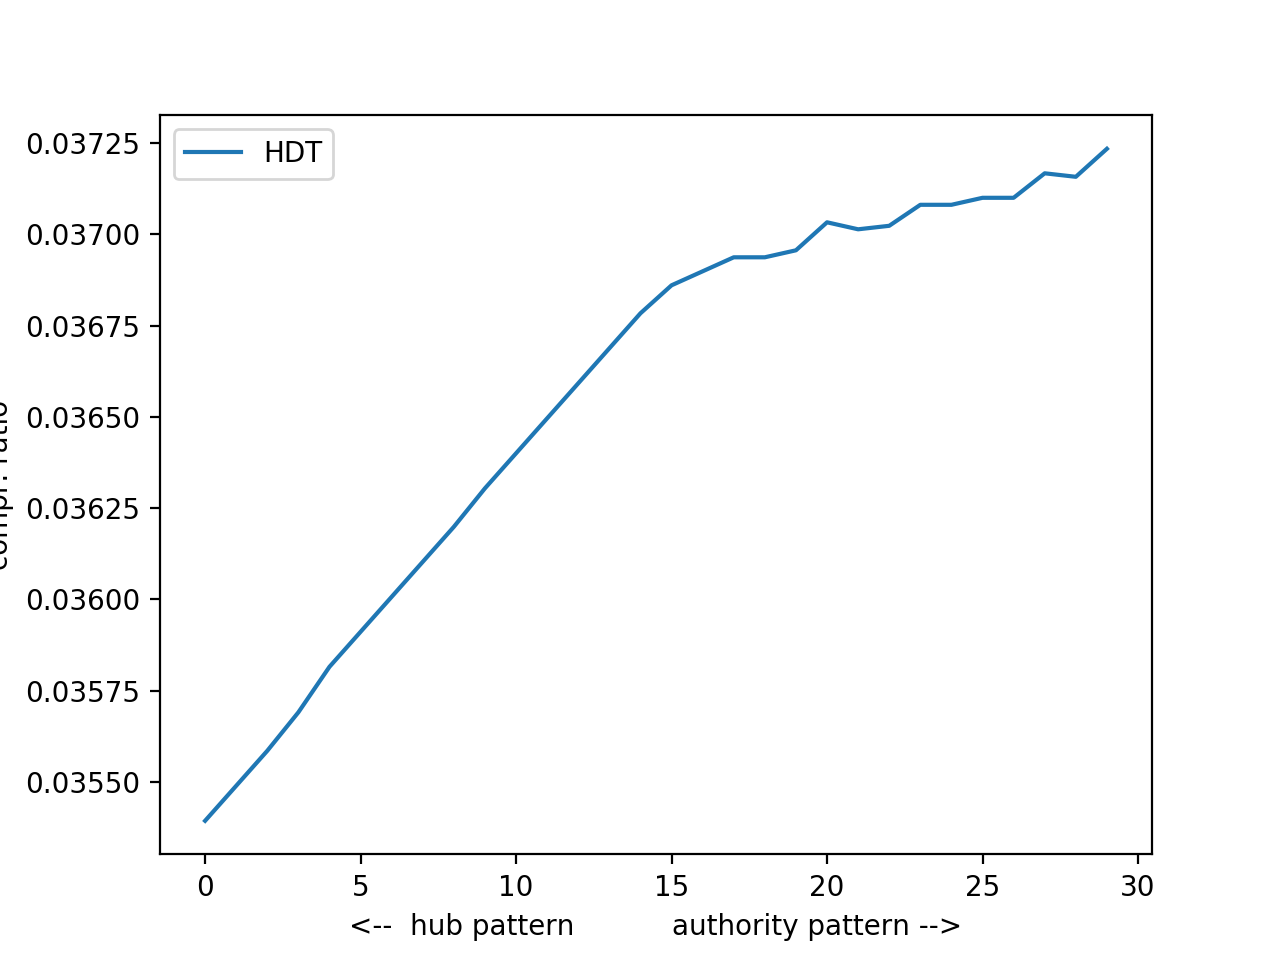
\includegraphics[width=0.5\textwidth]{figures/GRPvsHDT/hdtWithoutDict}\label{fig:ratiosHDTWithoutDict}}
	\hfill
	\subfloat[With dictionary size.]{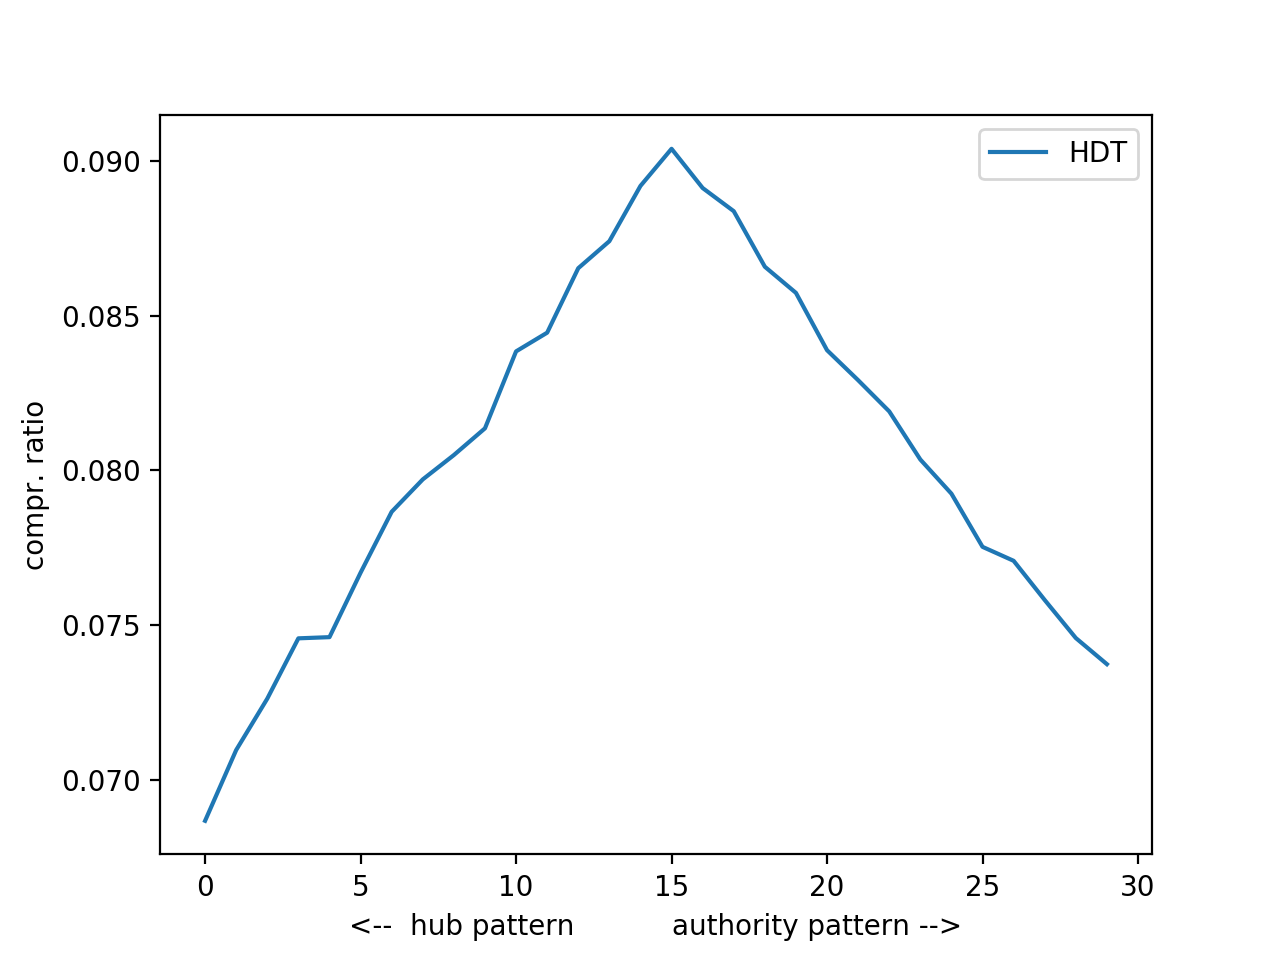
\includegraphics[width=0.5\textwidth]{figures/GRPvsHDT/hdtWithDict}\label{fig:ratiosHDTWithDict}}
	\caption{The compression ratios for HDT without and with dictionary sizes.}
\end{figure}

Next the compression ratio of GRP is considered, which is presented in Fig.~\ref{fig:ratiosGRPWithoutDict} (without dictionary sizes). Here one can see that GRP has a better compression ratio if the graph is more similar to the star pattern (hub order authority pattern). This property of GRP has also been mentioned in~\cite{maneth}. It can also be seen that the effect on the compression ratio is bigger for GRP than for HDT (standard deviation is twice as high for GRP as for HDT). A grammar-based compression is therefore more dependent on the structure of the input data.

When Fig.~\ref{fig:ratiosGRPWithDict} is considered, it can be seen that this curve behaves almost exactly like the one from Fig.~\ref{fig:ratiosHDTWithDict}, since the size of the dictionary accounts for most of the compressed data size.

\begin{figure}[h]
	\centering
	\subfloat[Without dictionary size.]{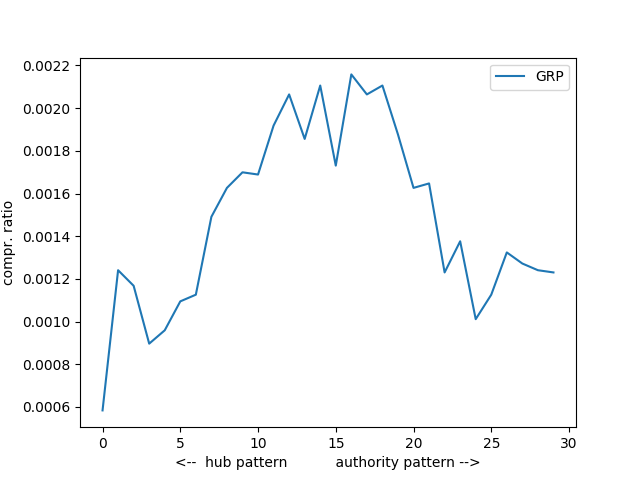
\includegraphics[width=0.5\textwidth]{figures/GRPvsHDT/grpWithoutDict}\label{fig:ratiosGRPWithoutDict}}
	\hfill
	\subfloat[With dictionary size.]{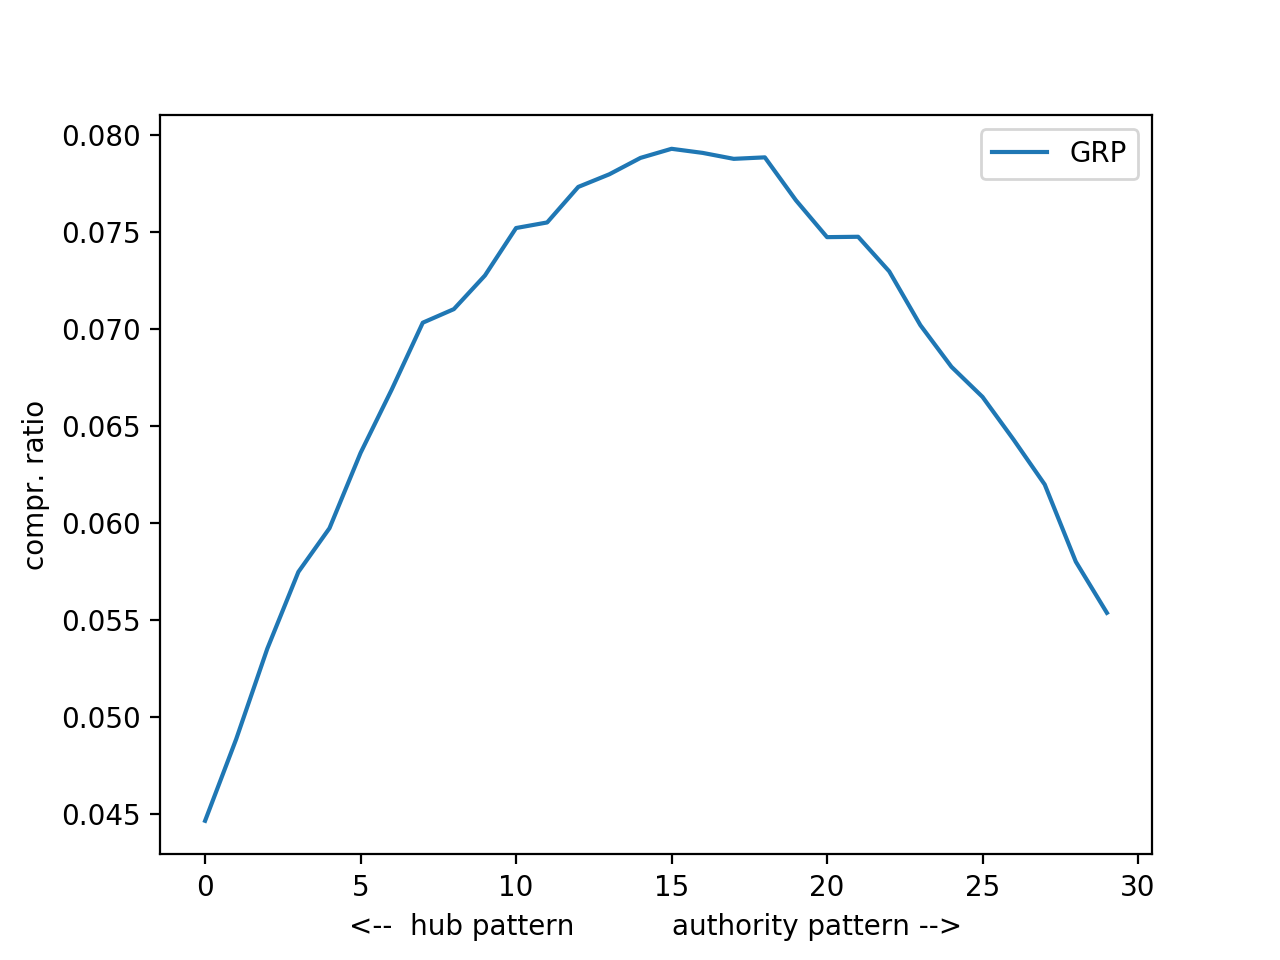
\includegraphics[width=0.5\textwidth]{figures/GRPvsHDT/grpWithDict}\label{fig:ratiosGRPWithDict}}
	\caption{The compression ratios for GRP without and with dictionary sizes.}
\end{figure}

Finally, Fig.~\ref{fig:ratiosBothWithoutDict} and Fig.\ref{fig:ratiosBothWithDict} show the compression ratios for both algorithms. Since both use the same method to compress the dictionary, the curves in Fig.~\ref{fig:ratiosBothWithDict} are very similar. However, it becomes clear that GRP compresses better than HDT. In Fig.~\ref{fig:ratiosBothWithoutDict}, the ratio of HDT is 31 times higher on average. Of course, this factor becomes much smaller in Fig.~\ref{fig:ratiosBothWithDict} because the dictionary accounts for most of the memory size. Here the compression ratio of HDT is on average 1.8 times as high as that of GRP.

\begin{figure}[h]
	\centering
	\subfloat[Without dictionary size.]{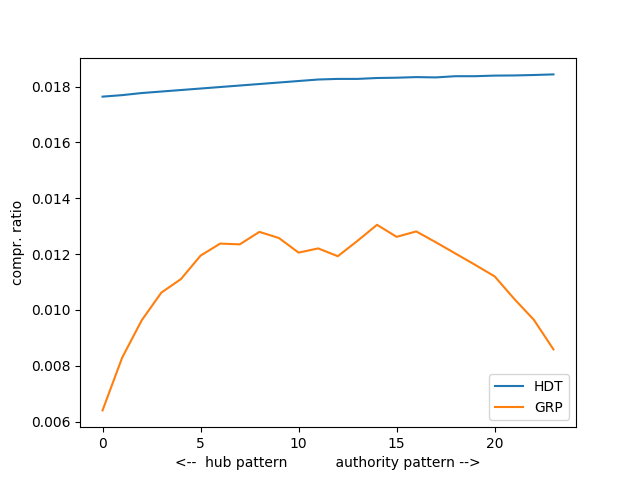
\includegraphics[width=0.5\textwidth]{figures/GRPvsHDT/bothWithoutDict}\label{fig:ratiosBothWithoutDict}}
	\hfill
	\subfloat[With dictionary size.]{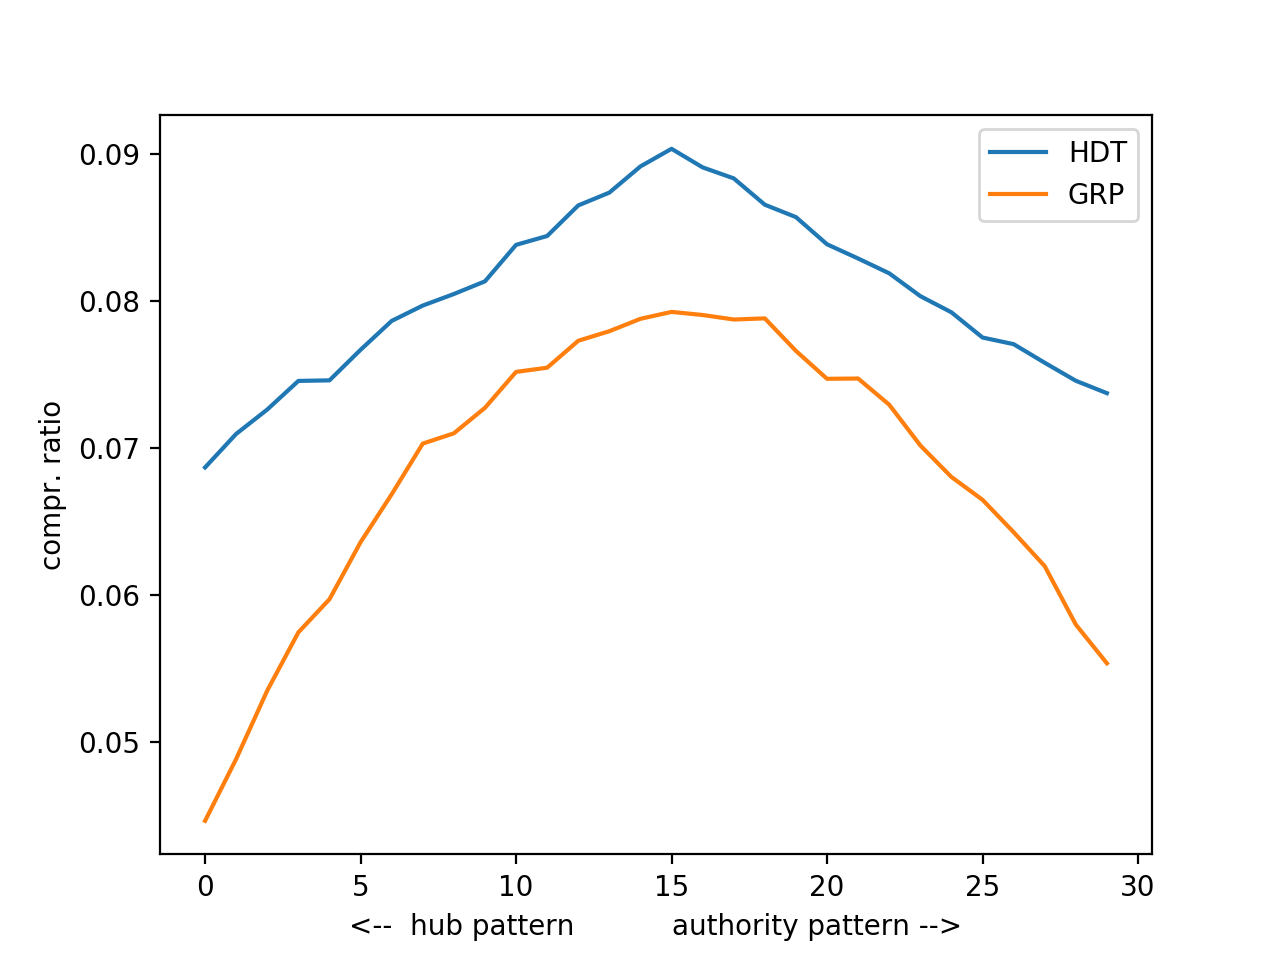
\includegraphics[width=0.5\textwidth]{figures/GRPvsHDT/bothWithDict}\label{fig:ratiosBothWithDict}}
	\caption{The compression ratios for GRP and HDT without and with dictionary sizes.}
\end{figure}

One could now argue that only one distinct predicate was used in that scenario and this is beneficial for GRP, as it gets worse as the number of predicates increases. Therefore a further evaluation is made in Fig.~\ref{fig:bothwithdict1000predicates}, where 1000 distinct predicates have been used. That is a quite high number considering the number of triples (1199) compared to real RDF data \todo{belegen}. One can see that the compression ratios are now higher for both compressors, but still GRP's ratio is always smaller than HDT's. HDT's ratio is still 1.7 times higher on average. So, the increasing number of predicates has a similar effect on both algorithms.

\begin{figure}
	\centering
	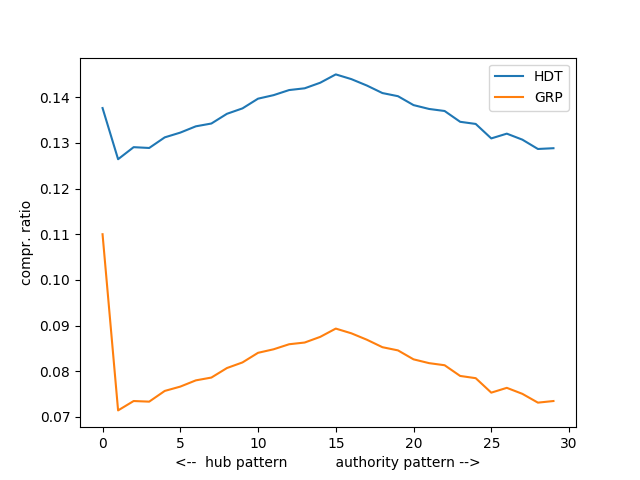
\includegraphics[width=0.7\linewidth]{figures/GRPvsHDT/bothWithDict1000Predicates}
	\caption{The compression ratios for GRP and HDT with dictionary sizes. Graphs have now 1000 distinct predicates.}
	\label{fig:bothwithdict1000predicates}
\end{figure}

Apart from the compression ratio, the run time is also important for the overall performance. Fig.~\ref{fig:runtimes} shows the average run times of the two algorithms. For this the same scenario with the star pattern (and only one distinct predicate) was used. It has been executed 100 times to get a sophisticated run time measurement, because the run time also depends on the current CPU workload of the computer.

\begin{figure}
	\centering
	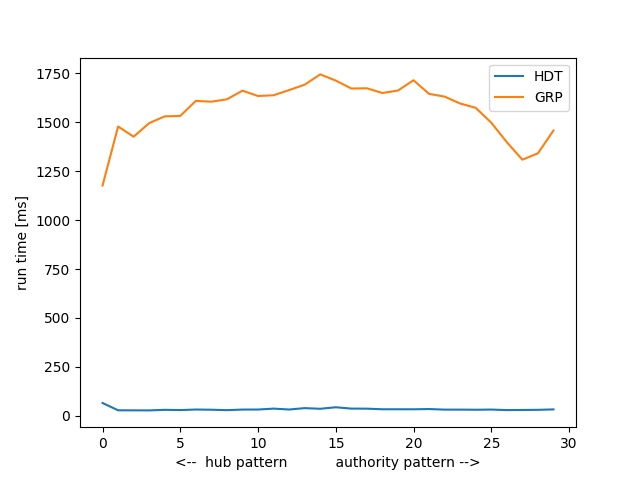
\includegraphics[width=0.7\linewidth]{figures/GRPvsHDT/runtimes}
	\caption{Run times of both algorithms (average run time of 100 consecutive executions).}
	\label{fig:runtimes}
\end{figure}


It can be seen that the runtime of GRP is significantly higher than that of GRP. It is on average ca. 48 times as high.

However, it should also be noted that the implementation of GRP is rather rudimentary  (according to the authors of~\cite{maneth}), while that of HDT has been under development for some time. So they are not comparable in terms of quality. Unfortunately, one cannot say at this point whether a more professional implementation of GRP will also be slower than HDT.

In addition one can notice that GRP's run time fluctuates more than that of HDT. GRP has a standard deviation of about 134, while HDT only has a standard deviation of about 7. One reason for this is that GRP, in contrast to HDT, is non-deterministic because of the partly random search order of the graph. On the other hand, the high deviations are also a confirmation of the above mentioned hypothesis that the behavior of GRP depends more on the structure of the input data than HDT does.



\section{Compression Improvements}

This chapter is about evaluating the compression improvements. It starts with applying ontology knowledge and then continues with dictionary compression improvement. In contrast to Ch.~\ref{sec:evaluationHDTvsGRP}, real data will be evaluated here to see how much influence the improvements have.

\subsection{Ontology Knowledge}\label{sec:evaluationOntKnowledge}

\subsubsection{Occurrence of Properties}
Now it will be presented how much of those symmetric/inverse/transitive properties exist in real data. For that we will use the datasets presented in Ch.~\ref{sec:implementationDatasets}. 

\begin{center}
\begin{tabular}{|c|c|c|c|}
	\hline 
	Dataset & Symmetric & Inverse & Transitive \\ 
	\hline 
	DBPedia &  &  &  \\ 
	\hline 
	Wordnet &  &  &  \\ 
	\hline 
	&  &  &  \\ 
	\hline 
\end{tabular}
\captionof{table}{The relevant properties for applying ontology knowledge found in real datasets.}	
\label{tab:properties}
\end{center}

Fig.~\ref{fig:ontoccurrences} shows how often the relevant properties occur in real datasets (DBPedia and Wordnet). (Relative amount = $\frac{\text{number of occurrences}}{\text{number of triples}}$). It can be noticed that the amounts are quite low, especially for symmetric and inverse properties. This supports the hypothesis from Ch.~\ref{sec:implementationOntKnowledge} that building sub graphs with higher amounts of relevant properties can be necessary to observe a real effect of the data manipulations. Nevertheless, first the normal datasets will be used to evaluate the manipulations.

\begin{figure}
	\centering
	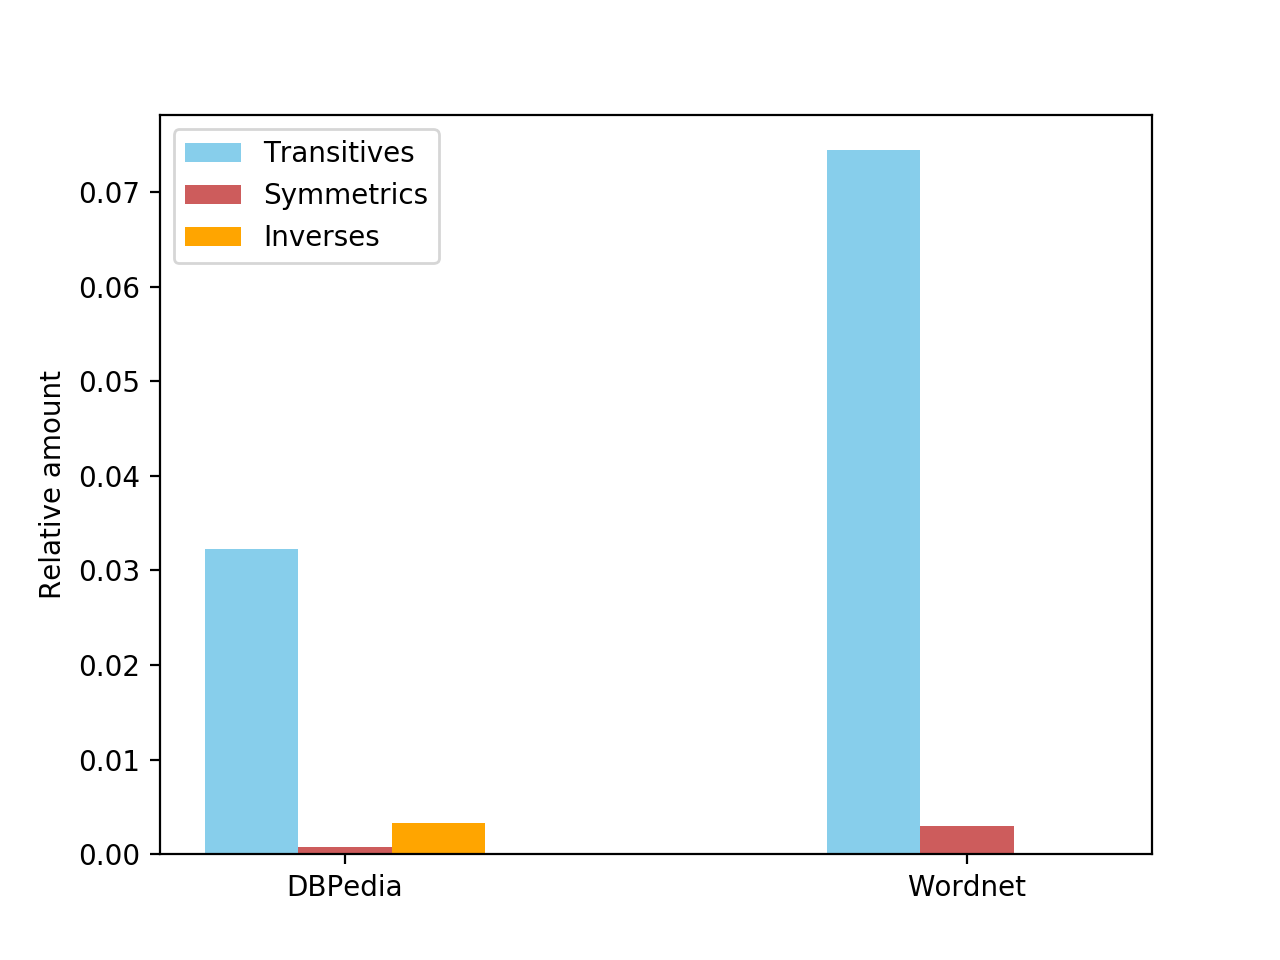
\includegraphics[width=0.7\linewidth]{figures/4_evaluation/ontOccurrences}
	\caption{Relative amount of transitive/symmetric/inverse properties in real datasets.}
	\label{fig:ontoccurrences}
\end{figure}




\subsection{Dictionary Improvements}\label{sec:evaluationDictImprovements}

At this point  about the evaluation of the approaches from Ch.~\ref{sec:implementationDictImprovements}. First the Huffman compression of literals is evaluated and then the compression of blank node IDs. Finally, both approaches combined will be evaluated.\todo{wurde das gemacht?}


\subsubsection{Literals}

As already mentioned, a self-generated Huffman code was used to compress the literals of an RDF graph, as one hopes for a better compression than the with the prefix-based compression of HDT.

Now the results of the evaluation are presented. First, the Semantic Web Dog Food data set is used. This is well suited for an evaluation, since both literals and URIS are included as objects. Fig.~\ref{fig:dogfoodcomprratios} shows the compression rates for a subset of the data (DF0 - DF9). 


\begin{figure}
	\centering
	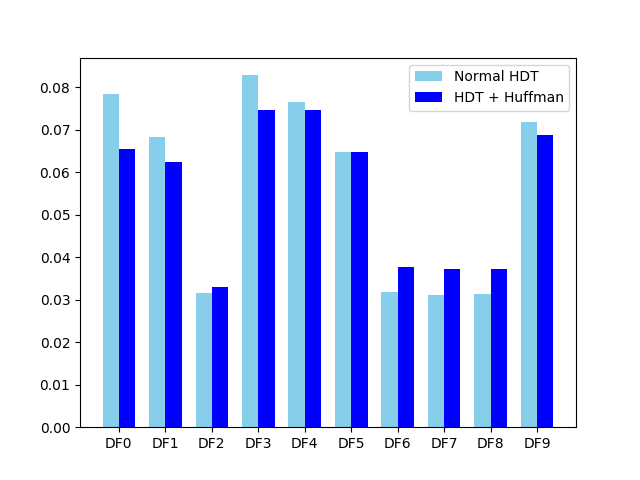
\includegraphics[width=0.7\linewidth]{figures/4_evaluation/dogFoodComprRatios}
	\caption{Compression ratios for Semantic Weg Dog Food Files. Comparison between Normal HDT and HDT + Huffman.}
	\label{fig:dogfoodcomprratios}
\end{figure}

One can see that the use of the Huffman code only brings a small improvement in some cases. In some cases Normal HDT even compresses better than HDT with Huffman.

This is because these data do not have a very high proportion of literals and literals are also rather short. This can be seen in Fig.~\ref{fig:dogfood}, where Fig.\ref{fig:dogfoodcomprratiosSub} lists compression rates again and Fig.\ref{fig:dogfoodliteralanalysis} shows the relative proportion of literals and the average length of a literal. The proportion of literals in the triples is never higher than 17.5\% and the highest average literal length is about 12. So these are single words rather than whole texts. Only in cases where both the proportion and the literal length are relatively high, an improvement can be seen (e.g. with DF9).


\begin{figure}[h]
	\centering
	\subfloat[Compression ratios for Normal HDT and HDT + Huffman]{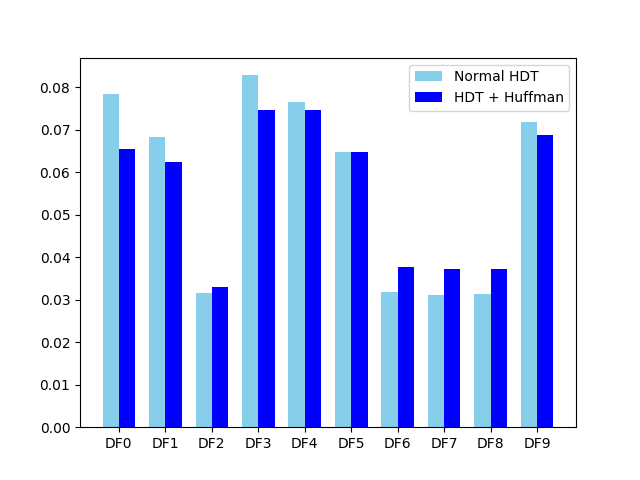
\includegraphics[width=0.5\textwidth]{figures/4_evaluation/dogFoodComprRatios}\label{fig:dogfoodcomprratiosSub}}
	\hfill
	\subfloat[Relative amounts of literals and average literal length.]{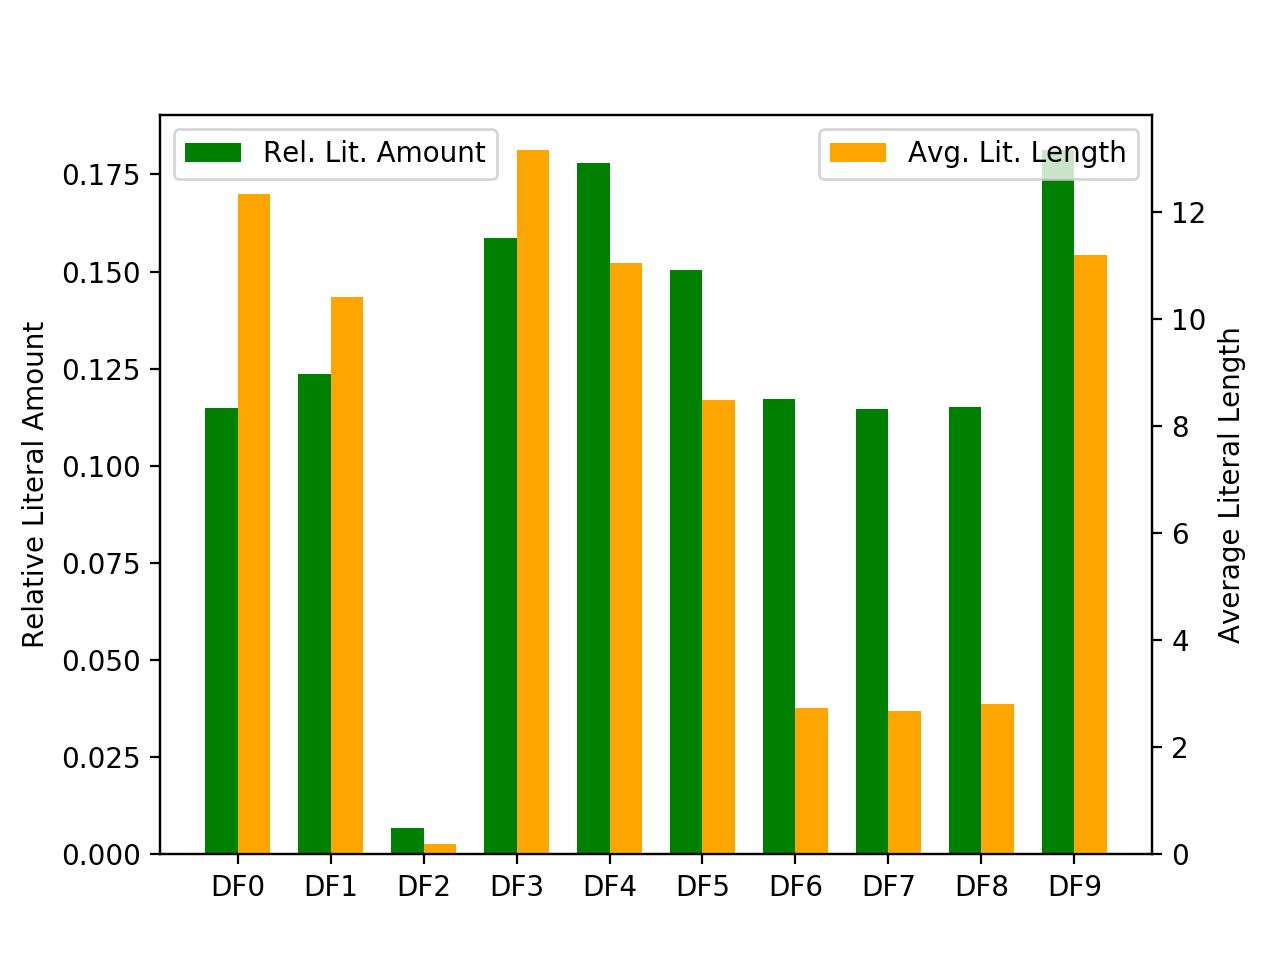
\includegraphics[width=0.5\textwidth]{figures/4_evaluation/dogFoodLiteralAnalysis}\label{fig:dogfoodliteralanalysis}}
	\caption{Relation between literal percentage and literal length (right) and compression ratios (left) for Semantic Web Dog Food Data.}
	\label{fig:dogfood}
\end{figure}

Now the DBPedia data set is considered, because it has a different structure of data. Here, graphs are considered which contain the abstracts of Wikipedia, because these are longer texts. In addition there are abstracts in different languages, so you can see if some languages are better suited for Huffman than others.

Fig.~\ref{fig:dbAbstractscomprratiosSub} shows the compression rates for the abstracts. The abbreviations stand for the languages in which the abstracts are written. It can be seen that Huffman significantly improves the compression rates here. The reason for this can be seen in Fig.~\ref{fig:dbAbstractsliteralanalysis}, where the average literal length is illustrated. The relative proportion of literals is not shown this time, since it is 100\% for all files. The average literal length varies between languages, but is generally much higher than in Semantic Web Dog Food. Therefore, the improvement is much greater here.

Another phenomenon can also be seen here: Although the English file contains by far the longest literals, the improvement by Huffman here is not as big as, for example, in the Bulgarian file. In the English case, the Huffman code is less effective because there are fewer different characters than in the other languages. Huffman is generally more efficient on large alphabets, according to~\cite{huffman}.

\begin{figure}[h]
	\centering
	\subfloat[Compression ratios for Normal HDT and HDT + Huffman]{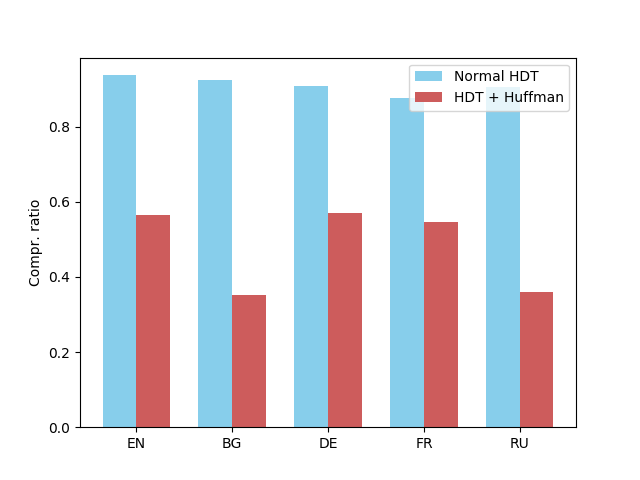
\includegraphics[width=0.5\textwidth]{figures/4_evaluation/dbAbstractsComprRatios}\label{fig:dbAbstractscomprratiosSub}}
	\hfill
	\subfloat[Average literal length.]{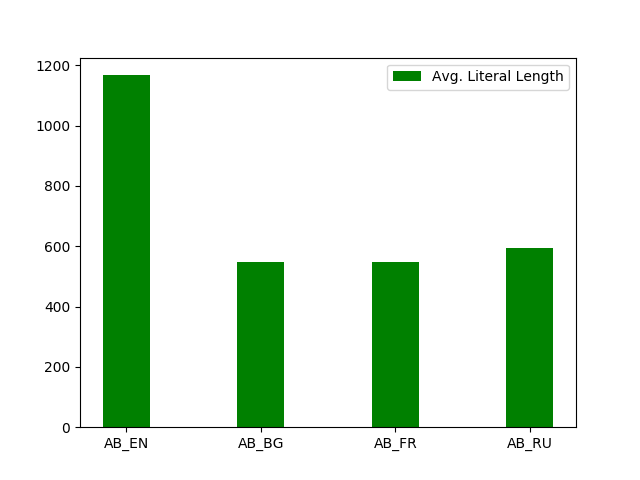
\includegraphics[width=0.5\textwidth]{figures/4_evaluation/dbAbstractsLiteralAnalysis}\label{fig:dbAbstractsliteralanalysis}}
	\caption{Relation between literal length (right) and compression ratios (left) for DBPedia Abstracts (Abbreviations denote the languages the abstracts are written in).}
	\label{fig:dbAbstracts}
\end{figure}

As mentioned above, saving the Huffman code means almost no additional storage effort. The average fraction of the Huffman code is about 0.1\% and was therefore not displayed in the visualizations.

Since the calculation of the Huffman code increases the runtime of the whole compression, it is now considered how big this effect is. Fig.~\ref{fig:dbAbstractsRuntimes} shows the run times for the compression of the DBPedia abstract data. Here the runtime has been increased very much. This is because HDT can normally compress very little with this data because of the many long literals and is therefore finished quite quickly. With Huffman one can compress much better and it takes quite a long time.

In Fig.~\ref{fig:dogFoodRuntimes} you can see the run times for the Semantic Web Dog Food data, where the run times are only slightly longer, because Huffman hardly improves the compression.

So it can be said that the use of a standard Huffman code could be worthwhile because of the otherwise high runtime. At this point, however, the evaluation with such a standard code was omitted, since such existing codes do not contain all the special characters that occur in RDF data.


\begin{figure}[h]
	\centering
	\subfloat[Run times for DBPedia abstracts.]{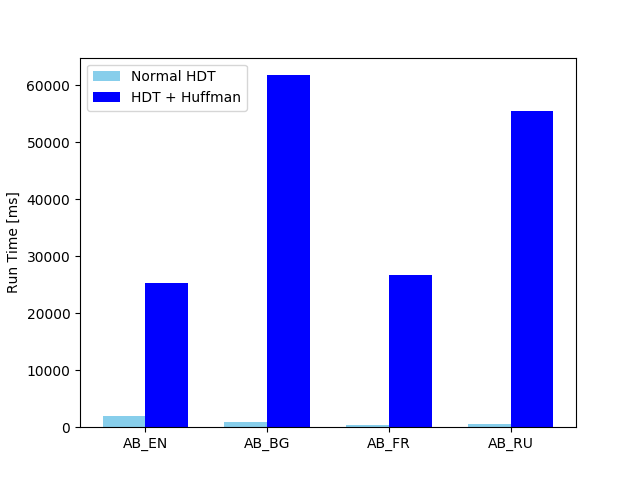
\includegraphics[width=0.5\textwidth]{figures/4_evaluation/dbAbstractsRuntimes}\label{fig:dbAbstractsRuntimes}}
	\hfill
	\subfloat[Run times for Semantic Web Dog Food files.]{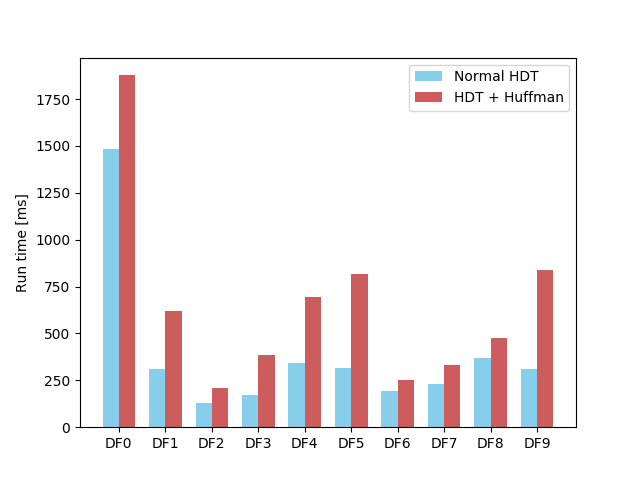
\includegraphics[width=0.5\textwidth]{figures/4_evaluation/dogFoodRuntimes}\label{fig:dogFoodRuntimes}}
	\caption{Run times for Normal HDT and HDT + Huffman.}
	\label{fig:huffmanRuntimes}
\end{figure}

\subsubsection{Blank Nodes}

\subsubsection{Literals and Blank Nodes Combined}

\subsection{Ontology and Dictionary}
\todo{evtl beides anwenden,wahrscheinl. ist ont Anteil so gering dass man es auf Grafik nicht sehen kann}






























